\chapter{Umsetzung}
\label{chap:umsetzung}

\section{Vorbemerkungen zum Renderer}
\label{sec:renderer}
Der Renderer wurde in JavaScript geschrieben da dies die einzige Programmiersprache ist, die clientseitig von jedem modernen Browser ohne manuellen Kompilierunsgprozess, Plugins oder ähnlichem ausgeführt werden kann. Da JavaScript einige Eigenheiten besitzt und für das Schreiben des Renderers eine bestimmte Designphilosophie und Bibliotheken verwendet wurde, werden diese zum besseren Verständnis des Codes im Folgenden erläutert.

\subsection{JavaScript}
JavaScript ist eine sehr ausdrucksstarke Sprache, die es dem Programmierer ermöglicht mit wenigen Codezeilen sehr elegante und schlanke Anwendungen zu schreiben. Allerdings hat JavaScript bei vielen bis heute auch einen negativen Ruf. Nachfolgend einige Gründe hierfür:
\begin{itemize}
    \item Einige Teile der Sprache sind für Programmierer die bisher mit klassischen Programmiersprachen (C/C++, Java, etc.) gearbeitet haben schwer verständlich und unintuitiv, wie Prototypische Vererbung, das komplette Fehlen von Klassen, die im Vergleich sehr geringe Anzahl an Objekten für bestimmte Aufgaben ("`Klassenbibliothek"') oder die Verwendung mancher Sprachkonstrukte, wie dem \textit{Date}-Objekt.
    \item Schon kleine Fehler, wie ein vergessenes Semikolon, ein vergessener \textit{new} Operator oder ein vergessenes \textit{var} bei der Deklaration von Variablen, können zu unvorhersehbarem Programmverhalten und schwer auffindbaren Fehlern führen. Anders als klassische Sprachen werden die drei genannten Aspekte vom Interpreter nicht als Fehler gehandhabt, sondern als gültiger Code verarbeitet da sie bereits beim Sprachdesign so eingebaut wurden.
    \item JavaScript kennt das Prinzip von Namespaces oder Packages nicht, sondern arbeitet mit globalen Variablen. Dies kann in Verbindung mit fremden JavaScript-Code zu ernsthaften Konflikten führen und macht die Entwicklung von komplexeren und größeren Anwendungen schwerer als in anderen Sprachen.
\end{itemize}
Trotz des schlechten Rufs hat JavaScript aber auch einige sehr gute Seiten, welche die Sprache wirklich attraktiv machen und die man in manchen etablierten Sprachen schnell vermisst. Nachfolgend eine (sehr kleine) Auswahl:
\begin{itemize}
    \item Funktionen sind Objekte erster Klasse. Das heißt, sie können eigenständig existieren, über Variablen referenziert und als Rückgabetypen von anderen und als Parameter in andere Funktionen zurückge-/übergeben werden. Funktionen können auch auch andere Funktionen als Attribute haben.
    \item Funktionen können als sogenannte Lambdafunktionen anonym verwendet werden. Dadurch müssen sie vor Gebrauch nicht erst benannt oder einer Variablen zugewiesen werden.
    \item Objekte können zur Laufzeit beliebig erstellt und um neue Attribute und Funktionen erweitert werden.
\end{itemize}
Der JavaScript-Guru Douglas Crockford hat ein Buch über die "`Good Parts"' (guten Seiten) der Sprache geschrieben \autocite{JsGoodParts}, in dem er auch die "`Bad Parts"' (schlechten Seiten) aufzeigt und Strategien erläutert, wie man diese möglichst elegant umgehen kann. Dieses Buch sei an dieser Stelle jedem empfohlen der sich etwas tiefer mit der Sprache beschäftigen oder einfach nur komplexere, wartbare Anwendungen damit entwickeln möchte.

ECMAScript\footnote{\url{http://www.ecmascript.org/} (besucht am \today)} ist der offizielle Name des Standards auf dem JavaScript aufbaut, und beide Begriffe werden häufig synonym verwendet. Jedoch ist JavaScript "`nur"' ein ECMAScript-Dialekt. Weitere Dialekte sind beispielsweise ActionScript\footnote{\url{http://www.adobe.com/devnet/actionscript.html} (besucht am \today)} von Adobe (bekannt für die Flashprogrammierung). Die Entwicklung von JavaScript schreitet kontinuierlich voran und wird derzeit vor allem durch HTML5 beschleunigt. JavaScript ist eine interpretierte Sprache, für die von jedem Browserhersteller eine Laufzeitumgebung eingebaut werden muss. Dies führt zwar einerseits dazu dass heutige Browser immer schnellere JavaScript-Egines mitliefern, andererseits jedoch sind nicht alle Sprachfeatures (insbesondere die neueren) in jedem Browser verfügbar. Für viele Webentwickler ist es ein Teil der täglichen Arbeit Code auch mit älteren Browsern kompatibel zu machen.

Mit den Versionen ECMAScript 5 und 6 werden viele Verbesserungen in die Sprache Einzug halten, von denen die aktuellen Versionen moderner Browser bereits einige unterstützen, wie den \textit{Strict Mode}. In diesem Modus wird die Verwendung einiger besonders fehlerträchtiger Sprachkonstrukte, wie die \textit{with}- und \textit{eval}-Statements als Fehler gewertet und der Code kann nicht ausgeführt werden. Dieser Modus hilft gerade durch seine Einschränkungen jedoch validen und wartbaren Code zu schreiben und meiner Einschätzung nach sollten neue Pojekte immer mit aktiviertem Strict Mode geschrieben werden. Hierbei wird empfohlen ihn innerhalb der hierarchisch höchsten Funktion zu deklarieren, um Konflikte mit nicht Strict Mode-fähigem Fremdcode zu vermeiden. Der Strict Mode wird über den einfachen String \textit{"`use strict"'} aktiviert. Hierdurch können auch ältere Browser, die ihn nicht unterstützen, den Code ausführen da das Statement nur ein einfacher String ist. In Osiris ist jedes Modul im Strict Mode geschrieben.
\lstset{language=JavaScript}
\begin{lstlisting}[caption={Aktivierung des \textit{Strict Mode}}]
function doSomething() {
"use strict"

// rest of the code
}
\end{lstlisting}
Um einige der negativen Seiten zu beheben, oder dem Programmierer zumindest Möglichkeiten an die Hand zu geben sie zu vermeiden, sind vor allem im Laufe der letzten Jahre eine große Menge verschiedener JavaScript-Frameworks und Bibliotheken veröffentlicht worden. Darunter finden sich sowohl umfassende Alleskönner wie das Dojo Toolkit\footnote{\url{http://dojotoolkit.org/} (besucht am \today)} als auch sehr raffinierte Werkzeuge für spezielle Aufgaben, wie die AsyncJs-Bibliothek\footnote{\url{https://github.com/caolan/async} (besucht am \today)}.

Für die Umsetzung des WebGL-Renderers wurden ebenfalls einige Bibliotheken verwendet die teilweise auch die Architektur der Anwendung mitbestimmt haben. Um den Code zu verstehen ist es daher notwendig diese kurz vorzustellen.

\subsection{RequireJs}
RequireJs versucht das aus etablierten Sprachen nicht mehr wegzudenkende Konstrukt der Namensräume in JavaScript nachzubilden. Hierbei werden funktionale Komponenten in sogenannte "`Module"' verpackt, die von anderen Modulen abhängig sein können (ähnlich dem \textit{import}-Statement in Java) und anderen Modulen eine öffentliche Schnittstelle für den Umgang mit dem Modul bereitstellen. Dies verbessert die Codeorganisation enorm. Zudem übernimmt RequireJs das asynchrone Laden von benötigten Modulen, was zu einer Reduzierung des benötigten Codes führen kann und das Laden beim Seitenaufruf beschleunigt. Die Entwickler von RequireJs haben hierfür den Begriff \textit{Asynchronous Module Definition} (kurz AMD) eingeführt. Mittlerweile sind auch andere JavaScript-Bibliotheken nach diesem Muster aufgebaut oder bieten das Laden von nach AMD geschriebenen Modulen an.
\lstset{language=JavaScript}
\begin{lstlisting}[caption={Aufbau eines Moduls nach AMD in Osiris}, label={lst:amd}]
define(["zepto"], function($) {
  "use strict";

  function _visit(node, executor) {
    // private method. Only accessible inside this module
  }

  return {
    execute: function(traversableScene, executor) {
      // public method. Is part of the module's API
    }
  };
});
\end{lstlisting}
Der Code in Listing \ref{lst:amd} definiert ein namensloses (empfohlen) Modul mit den Abhängigkeiten auf das Modul \textit{zepto}. Abhängigkeiten werden immer als Strings in einem Array am Anfang der \texttt{define}-Funktion angegeben. Um auf die Module zugreifen zu können werden Referenzen auf sie in der folgenden anonymen Funktion an das Modul übergeben. Die Referenzen können auch anders heißen als das Modul selbst. Im vorliegenden Code wird das Modul \textit{zepto} über den Namen \textit{\$} referenziert. Dadurch ist es möglich auf öffentliche Egenschaften und Methoden dieses Moduls zuzugreifen. Das \texttt{return}-Statement gibt ein Objekt mit der öffentlichen API des Moduls zurück, über welche andere Module mit diesem Modul interagieren können (in diesem Falle nur die \texttt{execute}-Methode).

Statt in der HTML-Seite nun jede JavaScript-Datei einzeln zu referenzieren, legt man lediglich einen \texttt{<script>}-Tag an, in welchem RequireJs geladen und die Hauptausführungsdatei (Main) der Anwendung referenziert wird.
\lstset{language=HTML}
\begin{lstlisting}[caption={Referenzierung einer RequireJs-Anwendung in einer Play! Framework Template}, label={lst:requireJsInPlayreferenzieren}]
<script data-main="assets/javascripts/main" src="@routes.Assets.at("javascripts/lib/require.js")"></script>
\end{lstlisting}
Bei dem Code in Listing \ref{lst:requireJsInPlayreferenzieren} ist zu beachten, dass dies die Einbettung in der View Template des Play! Frameworks darstellt. Mehr dazu folgt im Kapitel \ref{chap:konzeption} \textit{Konzeption}.

Die über das \texttt{data-main} Attribut referenzierte Datei enthält nun die Konfiguration der verfügbaren Module.
\lstset{language=JavaScript}
\begin{lstlisting}[caption={Konfiguration der verfügbaren Module}, label={lst:konfigurationModule}]
require.config({
  // Non AMD scripts that add themselves to the global object
  shim: {
    "async": {
      exports: "async"
    },
    "zepto": {
      exports: "$"
    }
  },

  paths: {
    // app
    Osiris: "Osiris",

    // libraries
    zepto: "lib/zepto",
    async: "lib/async",

    ...

    // infrastructure
    SendMessage: "infrastructure/SendMessageToServer",

    ...
  }
});
\end{lstlisting}
Hierbei werden die Module benannt und der relative Pfad angegeben, unter dem die Moduldatei liegt (ohne die Endung \texttt{.js}). Bibliotheken, die nicht dem AMD-Schema folgen können über das \texttt{shim}-Objekt dennoch als solche behandelt werden.

RequireJs bietet noch einige Funktionen mehr, beispielsweise das Optimieren und Zusammenführen aller Module in einer Datei für das schnellere Laden, von denen ich allerdings im Rahmen dieser Arbeit keinen Gebrauch gemacht habe. Ohne RequireJs wäre es jedoch sehr viel schwieriger geworden separierten und gut wartbaren Code zu schreiben.

\subsection{AsyncJs}
In JavaScript gab es lange keine Threads (außer dem eigenen Anwendungsthread). Lang laufende Skripte blockierten die Anwendung und konnten dazu führen, dass im Browser ein Timeout erzeugt wurde und der Anwender eine Nachricht erhielt, dass das Skript möglichweise nicht richtig funktioniert. Im Rahmen von HTML5 wird versucht diesen Missstand mit Hilfe eines neuen, noch in der Entwicklung befindlichen, Standards zu beheben, den \textit{Web Workers}. Diese bieten die Möglichkeit komplexere Aufgaben, wie das Herunterladen großer Dateien oder komplexe Berechnungen, in separaten Threads auszuführen.

Als Alternative zu den Web Workers hat sich das asynchrone Callback-Pattern etabliert. Da Funktionen in JavaScript Objekte erster Klasse sind, können sie auch an andere Funktionen als Parameter übergeben und innerhalb dieser aufgerufen werden. Hierdurch blockiert der Aufruf einer Funktion nicht die komplette Anwendung. Diese kann mit anderen Dingen fortfahren und kann über das registrierte Callback auf das Ergebnis der angestoßenen Funktion reagieren, obwohl alles nur in einem Thread abläuft. Dies nennt man \textit{reaktive} oder \textit{eventgetriebene} Programmierung.
\begin{figure}
\centering
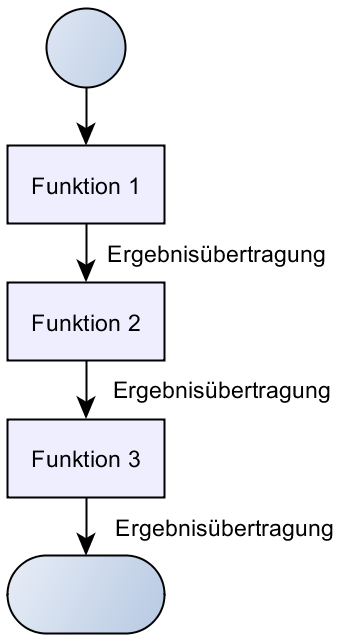
\includegraphics[height=80mm]{bilder/asyncwaterfall.png}
\caption{Beispielablauf der Funktion \texttt{waterfall} aus AsyncJs}
\label{fig:asyncwaterfall}
\end{figure}
Bei der Implementierung des Renderers fiel die Entscheidung aus pragmatischen Gründen für das Callback-Pattern, da für Web Worker erheblich mehr Aufwand betrieben werden muss und die vom Renderer parallel ausgeführten Tasks nicht so komplex sind, dass sie die komplette Anwendung einfrieren lassen können. Web Worker werden in einer eigenen, sehr abgeschotteten Umgebung ausgeführt in der nicht alle Möglichkeiten von JavaScript zur Verfügung stehen. Zudem ist die Integration mit RequireJs noch nicht auf unkomplizierte Weise gelöst.
\lstset{language=JavaScript}
\begin{lstlisting}[caption={Beispiel für eine Methode mit einem Callback}, label={lst:funktionmitcallback}]
function downloadFileFromUrl(url, callback) {
  var file;

  // download the file's contents into the file variable

  callback(file);
}
\end{lstlisting}
\lstset{language=JavaScript}
\begin{lstlisting}[caption={Beispiel für ein mögliches Callback}, label={lst:callbackbeispiel}]
var callback = function(file) {
  window.alert(file);
}
\end{lstlisting}
In Listing \ref{lst:funktionmitcallback} wird anhand einer einfachen Funktion gezeigt, wie am Ende einer Funktion das Ergebnis statt per \texttt{return} an den Aufrufer zurück, es an das registrierte Callback übergeben und dieses aufgerufen wird. Das Callback könnte dabei so aussehen wie in Listing \ref{lst:callbackbeispiel}, welches den Inhalt der Datei über eine Benachrichtigung auf dem Bildschirm darstellen würde.

Callbacks sind eine sehr gut Möglichkeit um mehrere Aufgaben parallel laufen zu lassen. Jedoch weiß man nie wann und ob ein Callback ausgeführt wird. Wenn die weitere Ausführung von Programmcode beispielsweise von den Ergebnissen mehrerer paralleler Aufgaben abhängig ist, muss vom Programmierer garantiert werden dass der nächste Schritt erst gestartet wird nachdem alle relevanten Callbacks ausgeführt wurden und ihre Ergebnisse geliefert haben.

Die AsyncJs-Bibliothek bietet hier Abhilfe. Über die in ihr enthaltenen Funktionen lassen sich auch komplexe asynchrone Abläufe sehr gut steuern. Zudem werden auch Funktionen angeboten mit denen Collections, wie Arrays und Objekte parallel verarbeitet werden können.
\lstset{language=JavaScript}
\begin{lstlisting}[caption={Beispiel für einen Aufruf von AsyncJs}, label={lst:asyncjsbeispiel}]
Async.waterfall([
  function(callback) {
    DownloadSceneFromServer.execute(sceneInformation, callback);
  },
  function(downloadedScene, callback) {
    PrepareSceneForRendering.execute(downloadedScene, glContext, callback);
  }
], _onComplete);
\end{lstlisting}
Wie Listing \ref{lst:asyncjsbeispiel} exemplarisch zeigt wird in der Regel ein Hauptcallback (\texttt{\_onComplete}) angegeben welches ausgeführt wird, sobald alle Funktionen ihr jeweiliges lokales Funktionscallback aufgerufen haben. Diesem Hauptcallback können aufgetretene Fehler oder erreichte Ergebnisse mitgegeben werden. Ein mögliches Hauptcallback ist in Listing \ref{lst:asyncjscallbackbeispiel} zu sehen. Die Abbildungen \ref{fig:asyncwaterfall}, \ref{fig:asyncparallel} und \ref{fig:asyncauto} zeigen den Ablauf von dreien der in der Bibliothek enthaltenen Funktionen.
\lstset{language=JavaScript}
\begin{lstlisting}[caption={Beispiel eines Hauptcallback für Listing \ref{lst:asyncjsbeispiel}}, label={lst:asyncjscallbackbeispiel}]
function _onComplete(error, preparedScene) {
  if (error) {
    throw error;
  }
  RenderScene.execute(preparedScene);
}
\end{lstlisting}
\begin{figure}
\centering
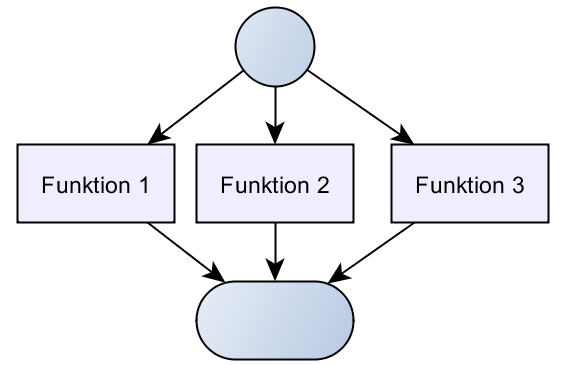
\includegraphics[width=70mm]{bilder/asyncparallel.png}
\caption{Beispielablauf der Funktion \texttt{parallel} aus AsyncJs}
\label{fig:asyncparallel}
\end{figure}
Für Osiris sind drei der AsyncJs-Funktionen von besonderer Bedeutung, denn sie bestimmten das Ablaufverhalten einiger Module maßgeblich:
\begin{enumerate}
    \item \textbf{async.parallel}\\
Führt gegebene Funktionen gleichzeitig (parallel) aus. Die Ergebnisse oder Fehler werden für jede beendete Funktion an das Hauptcallback geliefert. Dieses hat nun Zugriff auf alle Ergebnisse.
    \item \textbf{async.waterfall}\\
Führt gegebene Funktionen nacheinander aus und übergibt das Ergebnis der Vorgängerfunktion an die nachfolgende. Das Ergebnis der letzten Funktion wird an das Hauptcallback geliefert.
    \item \textbf{async.auto}\\
Erstellt einen Abhängigkeitsgraphen der registrierten Funktionen und führt sie so aus, dass Funktionen mit gleichen Abhängigkeiten parallel ausgeführt werden sobald die Abhängigkeiten erfüllt sind.
\end{enumerate}
Durch die Verwendung von AsyncJs war es möglich viele Vorgänge, wie das Herunterladen und Vorbereiten von Szene und Shaderprogramm, gleichzeitig ablaufen zu lassen und so die Verarbeitung zu beschleunigen. Zudem lassen sich mögliche Abhängigkeiten beispielsweise über die \texttt{async.auto}-Funktion sehr leicht beschreiben und die Verwaltung der verschiedenen Callbacks für jedes Modul über das Hauptcallback stark erleichtern. Denn eine besondere Schwierigkeit bei vielen Callbacks ist nicht den Überblick zu verlieren und so schwer auffindbare Fehler in den Programmcode einzubauen.
\begin{figure}
\centering
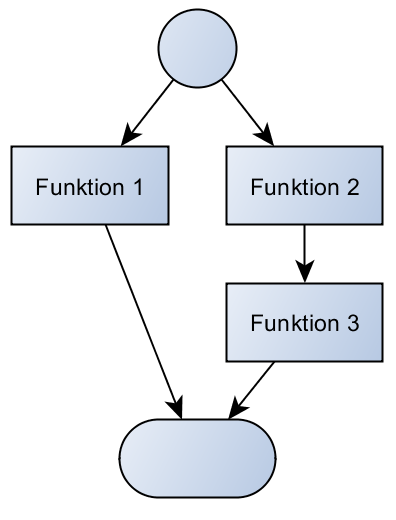
\includegraphics[height=70mm]{bilder/asyncauto.png}
\caption{Beispielablauf der Funktion \texttt{auto} aus AsyncJs}
\label{fig:asyncauto}
\end{figure}
\subsection{Weitere Bibliotheken}
Die restlichen Bibliotheken haben die Struktur des Renderer-Codes nicht maßgeblich beeinflusst, weshalb ihre Aufgaben nur kurz erwähnt werden.
\begin{itemize}
    \item \textbf{glMatrix}\\
GlMatrix ist eine speziell für WebGL entwickelte Matrizen- und Vektorenbibliothek. Mit ihr lassen sich komfortabel und sehr schnell allgemeine Berechnungen durchführen und sie enthält einige Funktionen die die Arbeit mit WebGL vereinfachen, wie \texttt{perspective} und \texttt{lookAt}.
    \item \textbf{WebGL Utils}\\
Eine von Google entwickelte Bibliothek die den Umgang mit dem WebGL-Kontext vereinfacht. Sie prüft automatisch ob der verwendete Browser WebGL beherrscht und erstellt eine Fehlerseite mit Informationen, falls nicht.
    \item \textbf{Log}\\
Ein kleiner selbstgeschriebener Wrapper für JavaScript-Logging. Wenn es im Browser kein \texttt{Console}-Objekt und daran bestimmte Methoden gibt, werden die Log-Nachrichten als Benachrichtigungsdialoge ausgegeben.
    \item \textbf{Zepto}\\
Zepto ist eine Bibliothek die hauptsächlich zur DOM\footnote{Document Object Model}-Manipulation gedacht ist und eine ähnliche API wie jQuery anbietet. Dabei ist sie aber deutlich kleiner als ihr Vorbild, da sie keine Unterstützung für alte Browser (z.B.: Firefox < Version 4) oder den Internet Explorer mitbringt.
\end{itemize}

\subsection{Flow Based Programming}
\begin{figure}
\centering
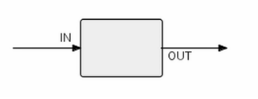
\includegraphics{bilder/fbp_component.png}
\caption{Schaubild einer Elementary Component \autocite{FlowBasedProgramming}}
\label{fig:fbpkomponente}
\end{figure}
In der klassischen Objektorientierung hat man Datenobjekte an denen Methoden (und unter Umständen auch Zustand) angeheftet sind, wie beispielhaft in Listing \ref{lst:ooptextdateibeispiel} zu sehen.
\lstset{language=JavaScript}
\begin{lstlisting}[caption={Beispiel für das objektorientierte Umbrechen einer Textdatei in JavaScript}, label={lst:ooptextdateibeispiel}]
var textFile = new TextFile();
textFile.load("some_text.txt");
textFile.wrapAtLine(80);
var success = textFile.save("wrapped_text.txt");

if (success) {
  window.alert("Text was read, wrapped and saved.");
} else {
  window.alert("Text could not be read, wrapped, and saved.");
}
\end{lstlisting}
Dies wirft einige Probleme auf, da hierbei verschiedene Aspekte zusammengeworfen werden. Das Objekt verletzt das Separation of Concerns-Prinzip, es "`tut"' zu viel: Zuerst greift es lesend auf das Dateisystem zu, liest den Inhalt der referenzierten Textdatei aus, bricht ihn um und speichert den modifizierten Inhalt wieder im Dateisytem. Zudem muss der Programmierer definitiv wissen in welcher Reihenfolge die Methoden des Objekts aufgerufen werden müssen. Im Beispiel ist es noch eine kleine Klasse. In der realen Welt entstehen jedoch oft sehr große Klassen die verschiedenste Aspekte in sich vereinen. Oftmals fällt es auch neuen Teammitgliedern schwer sich in die Architektur bereits bestehender Projekte einzulesen, da beispielsweise ein "`ResourceManager"' nicht auf den ersten Blick verrät welche Aufgaben tatsächlich über ihn abgewickelt werden.

Das Konzept des \textit{Flow Based Programming} (kurz FBP) wurde bereits in den späten 1960er Jahren von John Paul Morrison entwickelt und gewinnt heute durch die immer wichtiger werdende Nebenläufige Pogrammierung und die steigende Komplexität der zu entwickelnden Anwendungen wieder an Gewicht. Es unterscheidet sich in grundlegender Weise von der objektorientierten Herangehensweise, da hierbei nicht Datenstrukturen sondern funktionale Komponenten im Vordergrund stehen. Im FBP werden funktionale Einheiten als Black Box-Komponenten über ihr Verhalten und die eingehenden und ausgehenden Datenflüsse beschrieben. In Abbildung \ref{fig:fbpkomponente} wird eine einzelne Komponente dargestellt. Oftmals verfügen FBP-Komponenten lediglich über einen Ein- sowie Ausgang, können aber beliebig viele davon aufweisen. Jedoch sollte man hierbei strikt im Hinterkopf behalten, dass die Komponente als Ziel nur den zu erfüllenden Aspekt hat. Auf diese Weise sind sie so sehr leicht austausch- und in anderen Kontexten wiederverwendbar. Zudem erlauben sie dem Programmierer sich auf die Algorithmen für das Erledigen einer Aufgabe, sowie die Datenflüsse und die notwendigen Transformationen zu konzentrieren und verletzen die Clean Code-Prinzipien nicht.

Komponenten können auch andere Komponenten enthalten um ihre Aufgabe zu erledigen. Sie exportieren dieselben Schnittstellen wie einfache Komponenten, verbinden diese intern miteinander und dienen dem Programmierer so als Fassade zum komplexeren Vorgang. Diese Art von Komponente wird als \textit{Composite Component}, einfache Komponenten hingegen als \textit{Elementary Component} bezeichnet \autocite{FlowBasedProgramming}.\\
In Abbildung \ref{fig:fbpkomponenten} wird eine mögliche Composite Component dargestellt.
\begin{figure}
\centering
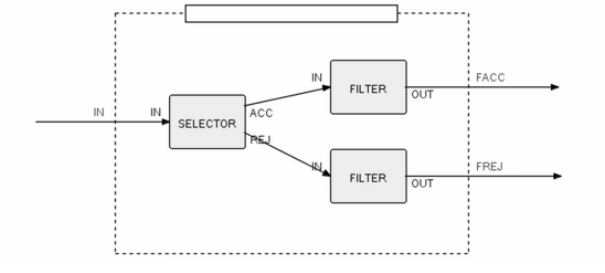
\includegraphics{bilder/fbp_components.png}
\caption{Schaubild einer Composite Component \autocite{FlowBasedProgramming}}
\label{fig:fbpkomponenten}
\end{figure}
Listing \ref{lst:fbptextdateibeispiel} zeigt den gleichen Vorgang wie im objektorientierten Beispiel in Listing \ref{lst:ooptextdateibeispiel} mit Flow Based Components.
\lstset{language=JavaScript}
\begin{lstlisting}[caption={Beispiel für das flussbasierte Umbrechen einer Textdatei in JavaScript}, label={lst:fbptextdateibeispiel}]
function WrapTextFileDemo() {
  var _readText,
    _wrapText,
    _saveText,

    _destPath,
    _wrapAtLine;

  _setup();
  _wire();

  function _setup() {
    _readText = new ReadTextFile();
    _wrapText = new WrapText();
    _saveText = new SaveTextFile();
  }

  function _wire() {
    _readText.onDone = function(readText) {
      _wrapText.execute(readText, _wrapAtLine);
    };

    _wrapText.onDone = function(wrappedText) {
      _saveText.execute(wrappedText, _destPath);
    };

    _saveText.onDone = function(success) {
      if (success) {
        window.alert("Text was read, wrapped and saved.");
      } else {
        window.alert("Text could not be read, wrapped, and saved.");
      }
    };
  }

  this.execute = function(sourceTextFilePath, destinationTextFilePath, wrapAtLine) {
    _wrapAtLine = wrapAtLine;
    _destPath = destinationTextFilePath;

    _readText.execute(sourceTextFilePath);
  };
}

var wrapTextFile = new WrapTextFileDemo();
wrapTextFile.execute("some_text.txt", "wrapped_text.txt", 80);
\end{lstlisting}
Der Code in Listing \ref{lst:fbptextdateibeispiel} zeigt, dass jede Aufgabe von einer spezialisierten Komponente übernommen wird. Diese werden, ähnlich wie in einem Baukastensystem, über ihre Ein- und Ausgänge miteinander verbunden, im Beispiel durch die private Methode \texttt{\_wire} ("`verdrahten"') realisiert. Wenn die erste Komponente \texttt{readText} ausgeführt wird "`fließen"' (daher auch der Name \textit{Flow Based}) die Daten durch die Komponenten hindurch und werden transformiert, bis am Ende das gewünschte Ergebnis erreicht ist. Alle Komponnenten bieten hierbei zum Start die \texttt{execute}-Methode an, der die notwendigen Parameter mitgegeben werden. Dies hat sich als Vereinbarung bewährt.

In obigem Beispiel ist zu sehen, dass sich die FBP-Komponenten in JavaScript mit objektorientierten Möglichkeiten implementieren und mit Callbacks als Ausgänge auch asynchron ausführen lassen. In diesem Fall wurden der Verständlichkeit halber alle Ausgänge \texttt{onDone} genannt. Über diese werden die Ergebnisse der in den einzelnen Komponenten durchgeführten Vorgänge nach außen mitgeteilt. Die Hauptkomponente \texttt{WrapTextFileDemo} ist als Composite Component realisiert und gibt den Erfolgsstatus am Ende direkt im Browser aus.

Für das Verständnis des Codes des Osiris-Renderers sollte diese kurze Einführung ausreichen. John Paul Morrison hat ein Buch über FBP geschrieben, welches das Paradigma sehr detailliert beschreibt \autocite{FlowBasedProgramming}.

\section{Vorbemerkungen zur Webanwendung}
Als Plattform für die Webanwendung und WebSocket-Server wurde das Play! Framework eingesetzt. Ein Framework für die Webanwendung einzusetzen war der schnellste Weg um die benötigte Serverinfrastruktur aufzubauen sowie die Implementierung und Anbindung des Renderers an SIRIS vornehmen zu können. Das Play! Framework bietet hierbei eine, im Gegensatz zu vielen etablierten Java oder Scala Web Frameworks, fast konfigurationsfreie Ausgangsbasis und enthält alle benötigten Konstrukte. Im folgenden Abschnitt werden die für Osiris relevanten Bestandteile kurz erläutert.

\subsection{Play! Framework}
Das Play! Framework ist für die Erstellung von modernen Webanwendungen in Java oder Scala entwickelt worden. Es ist es ein vollständig integriertes Paket in dem alles nötige, wie der Webserver und ORM-Mapper, bereits enthalten ist. Als Webserver wird Jetty (inklusive WebSocket-Protokoll) eingesetzt. Webanwendungen werden mittels des Model View Controller-Architekturmusters realisiert. In Version 2 ist der Quelltext von Java nach Scala portiert worden und die internen Klassen wurden auf das Akka\footnote{\url{http://akka.io/} (besucht am \today)} Actor-Framework umgestellt. Play! ist wie HTTP komplett statuslos, es müssen also alle relevanten Informationen bei jeder Anfrage mitgeschickt werden. Der Vorteil ist jedoch die sehr gute Skalierbarkeit. Da Version 2 noch sehr neu ist, ist die offizielle Dokumentation die Hauptreferenzquelle \autocite{PlayDoku}. Im Frühjahr 2013 werden wohl die ersten Bücher über Play! Version 2 in den Handel kommen\footnote{Der Verlag Manning Publications Co. wird je ein Buch für Java- und Scala-Entwickler herausgeben. \url{http://www.manning.com/hilton/} (besucht am \today)}.

HTTP-Anfragen werden vom Server angenommen und dann gemäß den Regeln in der \textit{routes}-Datei an einen Controller geleitet. Listing \ref{lst:playroutes} zeigt die Regeln für die Controller von Osiris. Hierbei wurde der \textit{Asset-Controller} ausgelassen. Dieser ist Teil des Frameworks und dient zum Herunterladen statischer Ressourcen über direkte Links. Von links nach rechts wird zuerst der akzeptierte HTTP-Anfragetyp deklariert. Dann die relative URL an die der Client anfragt und als letztes der angesprochene Controller und die öffentliche Methode, die ausgeführt werden soll.
\lstset{language=Scala}
\begin{lstlisting}[caption={Regeln für das Weiterleiten von HTTP-Anfragen an Controller}, label={lst:playroutes}]
GET   /         controllers.Application.index
POST  /shaders  controllers.ShaderController.getShaderConfigurationByFilename
POST  /scenes   controllers.SceneController.getSceneByFilename
GET   /socket   controllers.OsirisController.socket
\end{lstlisting}
Das Play! Framework bietet eine sehr leistungsfähige Template Engine. Statt wie in Version 1.x Groovy wird jetzt auch hier Scala verwendet. So können Datentypen vom Controller an die Template übergeben und dort in den HTML-Code eingebaut werden. Listing \ref{lst:playtemplates} zeigt ein Beispiel aus Osiris. Hierbei werden die Informationen zu den verfügbaren Szenen und Shaderprogrammen in ein HTML \textit{select}-Element (Dropdown-Box) integriert, sodass der Anwender später jeweils eins davon auswählen kann.
\lstset{language=HTML}
\begin{lstlisting}[caption={Integrieren der Informationen zu den verfügbaren Szenen und Shadern in ein HTML Select-Element}, label={lst:playtemplates}]
@(sceneInformation: Array[SceneInformation], shaderInformation: Array[ShaderConfiguration])

 ...

  <select id="availableScenes">
    @for(info <- sceneInformation) {
      <option value="@info.file">@info.name</option>
    }
  </select>

    ...

  <select id="availableShaders">
    @for(info <- shaderInformation) {
      <option value="@info.config">@info.name</option>
    }
  </select>
\end{lstlisting}
Für Osiris besonders relevant ist auch die JSON-Behandlung, denn alle ein- und ausgehenden Nachrichten sind so enkodiert. Das Framework bietet eine eigene JSON-Bibliothek an mit welcher es recht einfach ist JSON zu parsen oder zu erzeugen (siehe Listing \ref{lst:playjson}). Es können auch Reader und Writer für benutzerdefinierte Datentypen implementiert werden. Jedoch wurde aufgrund der wenigen benötigten Informationen hierauf verzichtet.
\lstset{language=Scala}
\begin{lstlisting}[caption={Erstellen und parsen eines JSON-Objekts}, label={lst:playjson}]
// Create JSON-Object from primitive values
val shaderInfo = Json.toJson(
  Map(
    "name" -> Json.toJson("Phong"),
    "vertexShader" -> Json.toJson(vertexShaderCode),
    "fragmentShader" -> Json.toJson(fragmentShaderCode),
    "bindables" -> Json.toJson(bindables)
  )
)

// Parse the created object
val name = (shaderInfo \ "name").as[String]
\end{lstlisting}
Eine Websocketverbindung aufzubauen ist sehr einfach. Hierzu werden die Datentypen \textit{Iteratee} und \textit{Enumerator} verwendet, die den Umgang mit Datenströmen abstrahieren. Iteratees werden zum Konsumieren des eingehenden Datenstroms verwendet, Enumeratoren für das Ausgeben der Nachrichten an den Client. Der Code in Listing \ref{lst:playwebsocket} stammt aus der offiziellen Play!-Doku\footnote{\url{http://www.playframework.org/documentation/2.0.3/ScalaWebSockets} (besucht am \today)}. Dort wird folgendes Verhalten gezeigt. Wenn sich ein Benutzer über ein Websocket mit dem Server verbindet, sendet dieser ein "`Hello!"' und schließt die Verbindung. Auf Serverseite wird hiernach zudem ein "`Disconnected"' auf der Konsole ausgegeben.
\lstset{language=Scala}
\begin{lstlisting}[caption={Empfangen und Senden über ein WebSocket in Play!}, label={lst:playwebsocket}]
def index = WebSocket.using[String] { request => 
  // Log events to the console
  val in = Iteratee.foreach[String](println).mapDone { _ =>
    println("Disconnected")
  }
  
  // Send a single 'Hello!' message
  val out = Enumerator("Hello!")
  
  (in, out)
}
\end{lstlisting}

\section{Anwendungsstruktur}
Beim Design von Osiris wurde darauf geachtet eine möglichst klare Struktur für das Projekt zu erreichen. Osiris besteht aus drei Teilprojekten: dem Play! Framework, SIRIS und der tatsächlichen Osiris-Anwendung. SIRIS und das Play! Framework liegen in ihren eigenen Ordnerstrukturen. Deren Code wurde, außer der bereits angesprochenen Abschaltung des Benchmarkings in SIRIS, im Original belassen. Alle für das Verständnis dieser Arbeit relevanten Dateien liegen im Projektordner \textit{osiris-play} (siehe Abbildung \ref{fig:playapp}). Dessen Struktur ist vom Play! Framework vorgegeben. Innerhalb dieser Ordnerhierarchie enthalten die folgenden Ordner den Quelltext für die Osirisanbindung und den Renderer:
\begin{itemize}
    \item \textbf{app}\\
Enthält alle serversetigen Klassen, wie die HTTP- und WebSocket-Controller, die Actors für die SIRIS-Anbindung und die HTML-Templates für die Gui des Renderers.
    \item \textbf{public}\\
Enthält alle statischen Ressourcen die vom Webserver ausgeliefert werden, wie CSS-Dateien, Szenen, Shaderprogrammcode, Modelle, Texturen und auch die JavaScriptmodule, die den Renderer ausmachen.
\end{itemize}
\begin{figure}
\centering
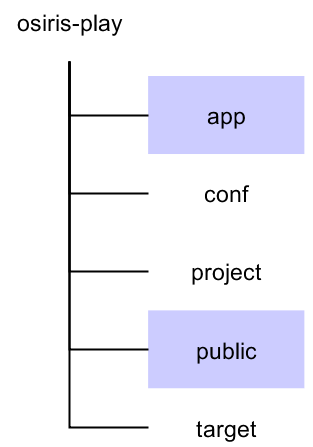
\includegraphics[height=60mm]{bilder/playapp.png}
\caption{Die Ordnerhierarchie der Anwendung. Blau markiert die besonders relevanten Ordner}
\label{fig:playapp}
\end{figure}

Bei der Programmierung wurde auf die Einhaltung der Clean Code-Prinzipien\footnote{\url{http://www.clean-code-developer.de/SOLID.ashx} (besucht am \today)}, wie beispielsweise \textit{DRY (Don't repeat yourself)} und \textit{SOC (Separation of Concerns)} geachtet. Aufgrund des Fehlens von Klassen in JavaScript, dem, im Gegensatz zu klassischen objektorientierten Sprachen, schwierigem Vererbungsmechanismus und der generell wünschenswerten Bevorzugung von Komposition vor Vererbung wurde für den Systementwurf das \textit{Flow Based Programming} (siehe Abschnitt \textit{Flow Based Programming}) eingesetzt. Für die SIRIS-Anbindung wurden Actors implementiert.

Die Module des Osiris-Renderers erfüllen alle eine spezielle Aufgabe und sind daher auch so benannt, beispielsweise \textit{DownloadSceneFromServer}. Alle Komponenten laufen asynchron und melden ihre Ergebnisse oder aufgetretene Fehler über registrierbare Callbacks als Ausgänge zurück. Dies verringert die Kopplung und erhöht die Wiederverwendbarkeit in anderen Projekten. Für die Rückgabe von Ergebnissen oder Fehlern wird in jedem Modul nur ein Callback registriert. Dies folgt der in AsyncJs vorgegebenen Form. Der erste Parameter ist immer ein etwaig aufgetretener Fehler oder \texttt{null}, wenn kein Fehler aufgetreten ist. Der zweite Parameter ist das Ergebnis. So ist es auch im NodeJS-Anwendungsframework\footnote{\url{http://nodejs.org/} (besucht am \today)} für welches AsyncJs ursprünglich entwickelt wurde.

Sowohl SIRIS als auch das Play! Framework verwenden zur Kompilation \textit{SBT (Simple Build Tool)}. Dies ist ein Werkzeug um die Erstellung von Scala-Projekten zu steuern, ähnlich wie \textit{Maven} oder \textit{Ant} für Java. Hierdurch konnte das SIRIS-Projekt Osiris einfach als Abhängigkeit hinzugefügt werden. Dadurch können in Osiris die SIRIS-Klassen importiert werden und bei der Kompilierung werden beide Projekte erstellt, zuerst SIRIS dann Osiris. Listing \ref{lst:osirissbtconfig} zeigt die Festlegung der Abhängigkeit.
\lstset{language=Scala}
\begin{lstlisting}[caption={Beschreibung der Abhängigkeit Osiris' von SIRIS in SBT}, label={lst:osirissbtconfig}]
lazy val siris = RootProject(file("../siris"))

val main = PlayProject(appName, appVersion, appDependencies, mainLang = SCALA).settings() dependsOn(siris) // Osiris depends on Siris
\end{lstlisting}

\section{Start von Osiris}
Beim Start der Anwendung wird zuerst der Jetty Server gestartet, auf dem das Play! Framework läuft. Darin werden die Controller für HTTP- und WebSocket-Requests, sowie die benötigten Actors für die SIRIS-Anbindung und die benötigten SIRIS-Actors selbst instanziiert.

Wenn der Benutzer nach dem Start der Anwendung die Url \texttt{http://localhost:9000} mit seinem Browser besucht, wird der Request an den \textit{Application}-Controller geleitet. Dieser erfüllt nun drei Aufgaben:
\begin{enumerate}
    \item Laden der Informationen zu den verfügbaren Shaderprogrammen
    \item Laden der Informationen zu den verfügbaren Szenen
    \item Einfügen der geladenen Informationen in das View-Template
\end{enumerate}
Die Informationen zu den verfügbaren Shaderprogrammen und Szenen finden sich in zwei vordefinierten JSON-formatierten Dateien, die im Dateisystem auf Serverseite liegen. Diese enthalten Metainformationen, wie Namen der Szenen und Shaderprogramme, die Pfade, wo die tatsächlichen Quelldateien gefunden werden können und im Falle der Shaderprogramme auch die bindbaren Attributes und Uniforms, mehr dazu etwas später. Diese Informationen werden gelesen, geparst, in das View-Template eingebaut und die fertige HTML-Seite anschließend an den Client ausgeliefert.

Alternativ zur Ablage im Dateisystem wäre der Einsatz einer dedizierten Datenbank möglich gewesen, welche die Informationen enthält. Der Einfachheit halber wurde jedoch hierauf verzichtet.

Sobald die HTML-Seite vom Client empfangen wurde, werden die verlinkte CSS-Datei und RequireJs geladen, welches seinerseits die im \texttt{data-main}-Attribut der HTML-Seite referenzierte Datei \textit{main.js} lädt und parst. In dem an \texttt{require.\-config} übergebenen anonymen Objekt befinden sich alle relevanten Informationen für RequireJs, um die Abhängigkeiten der benötigten Module aufzulösen und diese dann asynchron herunterzuladen. Im Anschluss wird das Modul \textit{Osiris} geladen und dessen \texttt{init}-Methode aufgerufen. Dieses Modul übernimmt nun drei Aufgaben:
\begin{enumerate}
    \item Initialisierung der Anwendung
    \item Kontrolle über das die grafischen Benutzeroberfläche manipulierende Viewmodel 
    \item Delegation der Anwendereingaben
\end{enumerate}
Das Layout und der Stil der grafischen Benutzeroberfläche werden in der HTML-Datei, respektive der \textit{main.css} festgelegt. Um jedoch eine klare Trennung von Layout/Stil und Anwendungscode zu erhalten, wurde ein separates Modul namens \textit{MainViewModel.js} im Ordner \textit{view} implementiert, welches sich an die HTML-Elemente anbindet und Funktionen bereitstellt um mit diesen zu interagieren. Für eine browserunabhängige Anbindung wurden die Möglichkeiten der \textit{Zepto}-Bibliothek verwendet. Diese bietet komfortable Methoden um HTML-Elemente zu manipulieren oder Informationen zu extrahieren. Das ViewModel stellt sowohl die vom \textit{Application}-Controller in die HTML-Seite eingefügten Shaderprogramm- und Szeneninformationen über die beiden Methoden \texttt{getCurrentShader} und \texttt{getCurrentScene}, als auch den Canvas für das Rendering über \texttt{getRenderCanvas} zur Verfügung. Zudem enthält die Seite einen Bereich für Statusmeldungen, über den die Applikation den Anwender über zur Laufzeit anfallende Benachrichtigungen und Fehler informieren kann. Den Zugriff hierauf abstrahiert das ViewModel über die Methode \texttt{updateStatus}.

Nachdem der Anwender nun die gewünschte Szene und das gewünschte Shaderprogramm gewählt und mit einem Klick auf den \textit{Start}-Button bestätigt hat, wird die \texttt{execute}-Methode des Osiris-Moduls aufgerufen.

\section{Initialisierung des WebGL-Kontext}
Der WebGL-Kontext ist inherent wichtig für fast alle Vorgänge innerhalb der Anwendung. Daher wird dieser zuerst initialisiert. Wie bereits beschrieben ist der Name des Kontexts noch nicht in allen Browsern auf "`webgl"' standardisiert, weshalb hierfür die WebGL Utils-Bibliothek angewendet wird. Listing \ref{lst:webglkontextaufbauen} zeigt den Aufruf innerhalb des Osiris-Moduls \textit{SetupWebGlContext}.
\lstset{language=JavaScript}
\begin{lstlisting}[caption={Initialisierung des WebGL-Kontext}, label={lst:webglkontextaufbauen}]
var glContext = WebGl.setupWebGL(canvas);
\end{lstlisting}
Da der Kontext für die Anwendung verloren gehen kann wird in allen Modulen, die auf den ihn angewiesen sind, vor der weiteren Verarbeitung die Funktion \texttt{isContextLost} aufgerufen. Es ist möglich über einen EventListener auf den Verlust des Kontexts zu reagieren. Allerdings schlugen Versuche hierzu fehl, da das Event kurioserweise immer direkt auftrat und so die Anwendung nicht weiterarbeiten konnte und andererseits jedes Modul anders auf den verlorenen Kontext reagieren muss. Es konnte auch nach einer längeren Recherche nicht nachvollzogen werden, warum das Event sofort geworfen wurde.

\section{Laden des gewählten Shaderprogramms}
Auf Clientseite wird das Modul \textit{LoadShaderProgram} gestartet, welches die Shaderinformationen des vom Anwender gewählten Shaderprogramms verarbeitet und über das registrierte Callback das fertige Shaderprogramm-Objekt zurückliefert. Zu den Shaderinformationen gehören der Name des Shaderprogramms, sowie Name und relativer Pfad zu einer Konfigurationsdatei. Letztere enthält folgende Daten:
\begin{itemize}
    \item Name der Datei, die den Code des Vertexshaders enthält
    \item Name der Datei, die den Code des Fragmentshaders enthält
    \item Bindbare Attributes und Uniforms
\end{itemize}
Für das Abrufen der nötigen Daten des gewählten Shaderprogramms existiert auf der Serverseite ein eigener Controller namens \textit{ShaderController}. Zuerst sendet der Client die JSON-enkodierten Informationen an den Server. Der ShaderController empfängt die Nachricht, lädt die referenzierte Konfigurationsdatei, parst sie und lädt die darin referenzierten Quellcodedateien für die Shader. Diese Informationen werden dann in ein JSON-Objekt verpackt und an den Client zurückgesendet. Dieser hat nun alle benötigten Daten um das gewählte Shaderprogramm zu erstellen. Hierfür müssen zuerst die beiden Shader kompiliert und dann dem Programm hinzugefügt werden. Schlussendlich wird das Programm noch "`gelinkt"'. Linken ist C-Programmierern ein Begriff. Nach der Kompilierung müssen die einzelnen Bestandteile noch zu einer ausführbaren Datei verbunden werden. Ähnlich gilt dies auch für ein WebGL-Shaderprogramm. Damit das Programm schlussendlich verwendet werden kann, wird die Funktion \texttt{useProgram} mit dem gelinkten Shaderprogramm als Parameter aufgerufen.

\section{Laden der gewählten Szene}
Das Laden der vom Anwender gewählten Szene läuft ähnlich ab wie das Laden des Shaderprogramms. So werden auch hier die Informationen zur gewählten Szene an einen dedizierten Controller namens \textit{SceneController} übertragen, welcher dann die Szene selbst zurückgibt. Jedoch müssen zuerst einige der enthaltenen Knoten in ein für den Renderer verständliches Format umgewandelt und referenzierte Daten, wie 3D-Modelle und Texturen, nachgeladen und ihrerseits transformiert werden.

\subsection{3D-Modelle}
WebGL benötigt die modellrelevanten Daten, wie Vertices, Normalen oder Indizes als strikt typisierte Bufferobjekte. Daher wurden in JavaScript typisierte Array-Objekte (siehe \autocite{TypedArrays}) eingeführt, welche nur einen bestimmten Datentypen enthalten können, wie das \textit{Float32Array} oder das \textit{Uint16Array}. WebGL stellt zwei binäre Bufferobjekte bereit, AR\-RAY\-\_BUF\-FER und EL\-E\-MENT\-\_AR\-RAY\-\_BUF\-FER. Deren Inhalte können über diese typisierten Arrays manipuliert werden. Die typisierten Arrays fungieren hier als "`Sicht"' (View) auf den Buffer. Da dieser immer nur binäre Daten enthält, wird durch das Array beschrieben welche Art von Daten sich darin befinden.

Alle für das Rendering relevanten Daten müssen in WebGL-Bufferobjekte umgewandelt werden, wie Listing \ref{lst:webglbuffer} zeigt.
\lstset{language=JavaScript}
\begin{lstlisting}[caption={Erstellen eines WebGL-Buffers und Anbinden der Daten}, label={lst:webglbuffer}]
var buffer = _gl.createBuffer();
_gl.bindBuffer(_gl.ARRAY_BUFFER, buffer);
_gl.bufferData(_gl.ARRAY_BUFFER, new Float32Array(vertices), _gl.STATIC_DRAW);
_gl.bindBuffer(_gl.ARRAY_BUFFER, null);
\end{lstlisting}
Zuerst wird ein Bufferobjekt erstellt, dann als ARRAY\-\_BUFFER-Typ referenziert und anschließend über ein Float32Array mit Daten befüllt. In der letzten Zeile wird die Referenz auf den Buffer gelöst, um ungewollte Veränderungen zu vermeiden.
\begin{figure}
\centering
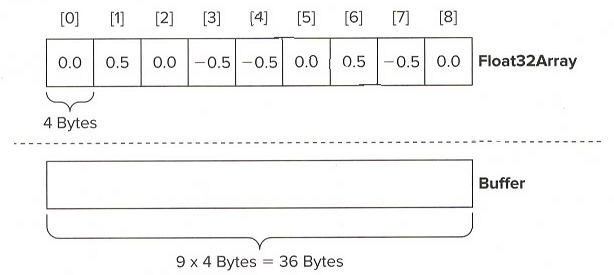
\includegraphics[width=100mm]{bilder/vbo.png}
\caption{Ein Bufferobjekt (unten) und die Float32Array-Sicht auf diesen Buffer (oben) \autocite{WebGlPogramming}}
\label{fig:vbo}
\end{figure}

\subsection{Texturen}
In der Szene werden Texturen als JPEG- oder PNG-Bilder referenziert. Diese können nicht direkt in WebGL verwendet werden sondern müssen zuerst umgewandelt werden. Dies ist mit Hilfe des in JavaScript vorhandenen \textit{Image}-Objekts sehr schnell umsetzbar. Dieses lädt die referenzierten Bilddateien asynchron herunter, was die gleichzeitige Verarbeitung mehrerer Bilder ermöglicht und somit die Vorbereitungszeit für das Rendering verkürzt. Über den in Listing \ref{lst:jsimageladen} gezeigten Code wird ein Bild von der angegeben Adresse heruntergeladen.
\lstset{language=JavaScript}
\begin{lstlisting}[caption={Herunterladen eines Bildes mit dem JavaScript Image-Objekt}, label={lst:jsimageladen}]
var image = new Image();

image.onload = function() {
  _handleLoadedImage(image, callback);
};

image.src = pathToImage;
\end{lstlisting}
Im \texttt{\_handleLoadedImage}-Callback wird dann die Erstellung einer WebGL-Textur durchgeführt. Listing \ref{lst:imageintextur} zeigt den Vorgang.
\lstset{language=JavaScript}
\begin{lstlisting}[caption={Umwandlung eines Image-Objekts in eine WebGL-Textur}, label={lst:imageintextur}]
function _handleLoadedImage(image, callback) {
  var texture = _gl.createTexture();

  _gl.bindTexture(_gl.TEXTURE_2D, texture);
  _gl.pixelStorei(_gl.UNPACK_FLIP_Y_WEBGL, true);
  _gl.texImage2D(_gl.TEXTURE_2D, 0, _gl.RGBA, _gl.RGBA, _gl.UNSIGNED_BYTE, image);
  _gl.texParameteri(_gl.TEXTURE_2D, _gl.TEXTURE_MAG_FILTER, _gl.LINEAR);
  _gl.texParameteri(_gl.TEXTURE_2D, _gl.TEXTURE_MIN_FILTER, _gl.LINEAR_MIPMAP_LINEAR);
  _gl.generateMipmap(_gl.TEXTURE_2D);

  _gl.bindTexture(_gl.TEXTURE_2D, null);

  callback(null, texture);
}
\end{lstlisting}
Zuerst wird eine WebGL-Textur erstellt, die Referenz darauf in der Variable \texttt{texture} gespeichert und als aktuell zu bearbeitende Textur gebunden. Der Aufruf der Funktion \texttt{pixelStorei(\_gl.UNPACK\-\_FLIP\-\_Y\-\_WEBGL, true)} dreht das Bild horizontal, da der Koordinatenursprung des Image-Objekts in der linken oberen Ecke, bei einer WebGL-Textur in der linken unteren Ecke liegt (siehe Abbildung \ref{fig:bilderkoordinatensysteme}).

Anschließend werden die Bytes des Bildes von der Funktion \texttt{texImage2D} aus dem Image-Objekt gelesen. Hierbei ist es wichtig anzugeben welche Farbkanäle das Bild enthält (RGB: Rot, Grün und Blau) und ob das Bild Transparenzen enthalten kann (Das A in RGBA steht für den Alphakanal). Für die visuelle Qualität sind zudem die Angaben für die Filterung der Textur notwendig. In diesem Beispiel wird die \textit{trilineare} Filterung verwendet. Um die Darstellungsqualität und die Leistung zu verbessern, können Mipmaps generiert werden (Funktion \texttt{generateMipmap}). Dies sind verkleinerte Repräsentationen des Originalbildes. Mit steigender Entfernung vom Betrachter zur Textur wird auf eine höhere Mipmapstufe umgeschaltet und nur noch das verkleinerte Abbild gezeichnet. Allerdings ist bei der Verwendung von Mipmaps zu beachten, dass die Größe der Textur dann ein Vielfaches von 2 sein muss (2, 4, 8, 16, 32 etc.). Höhe und Breite können sich unterscheiden (zum Beispiel: 128x512 Pixel). Am Ende des Beispiels wird über den erneuten Aufruf von \texttt{bindTexture} die Referenz auf die aktuelle Textur gelöst, um weitere Änderungen zu vermeiden.
\begin{figure}
\centering
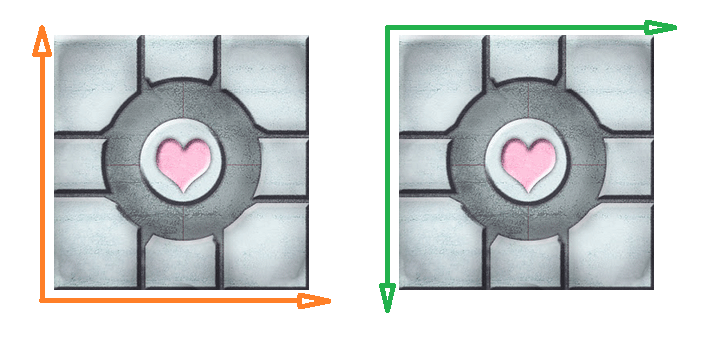
\includegraphics[width=\textwidth]{bilder/koordinatensysteme_bilder.png}
\caption{Links: Das Koordinatensystem einer WebGL-Textur, Rechts: Das Koordinatensystem des JavaScript Image-Objekts}
\label{fig:bilderkoordinatensysteme}
\end{figure}

Um die Texturen anzeigen zu können muss das 3D-Modell über Texturkoordinaten verfügen. Diese liegen wie bereits von OpenGL gewohnt zwischen 0 und 1. Für jedes Vertex wird ein Zweiertupel angegeben.

Osiris unterstützt zwei Texturtypen: Color Maps und Specular Maps (siehe Abbildung \ref{fig:texturemaps}). Color Maps enthalten die Farbinfomartionen, Specular Maps den Grad der Reflektivität für jedes Pixel. Je dunkler ein Pixel, desto weniger stark reflektiert das Licht an diesem Punkt. Weiß würde also volle Reflektion bedeuten, Schwarz gar keine.
\begin{figure}
\centering

\includegraphics[width=\textwidth]{bilder/texturemaps.png}
\caption{Links: eine Color Map, Rechts: die zugehörige Specular Map}
\label{fig:texturemaps}
\end{figure}

Hierbei ist zu beachten, dass alle Modellknoten die gleichen Arten von Texture Maps haben. Referenziert beispielsweise ein Modellknoten eine Specular Map in seinen Materialeigenschaften, sollten alle Modellknoten eine Specular Map referenzieren. Ansonsten kann es zu visuellen Artefakten kommen.

\section{Übertragen der Modellknoten an SIRIS}
Der Renderer sucht alle Modellknoten aus der Szene und sendet sie an den Server, welcher sie über die Anbindung an SIRIS der ebenfalls angebundenen Physikengine zugänglich macht. Für diese sind im Modellknoten seine physikalischen Eigenschaften, wie Masse, Reibungswiderstand, sowie Form und Größe der physikalischen Hüllform hinterlegt. Weiterhin benötigt die Physikengine die Transformationsmatrix des Objekts. Diese bestimmt sowohl die Position, als auch die Ausrichtung (Rotation) des Modells. Die Physikengine errechnet die physikalischen Kräfte, die auf das Objekt einwirken und aktualisiert dessen Transformationsmatrix. Der Renderer verwendet sie um das Objekt dann in der korrekten Position und Ausrichtung zu zeichnen.

\subsection{Vorbereitung der Datenübertragung}
Der Renderer extrahiert die Modellknoten über die Methode \texttt{byType} des Moduls \textit{FindNodes}. Diese liefert alle Knoten des Szenegraphen mit dem angegebenen Typen zurück, in diesem Fall mit dem Typen "`model"'.

Da die Kommunikation mit dem Server zu keinen unerwarteten Ergebnissen führen soll, wurden vorgefertigte Nachrichtentypen erstellt. Diese wandeln die über die Konstruktorparameter übergebenen Daten in eine vordefinierte JSON-Struktur um. Der Renderer kann zwei Nachrichtentypen an den Server senden:
\begin{enumerate}
    \item \textbf{SetupRequest}\\
Dient dem Senden von Modelknoten an SIRIS, für die es Entitäten erstellen und registrieren soll. Weiterhin sollen Veränderungen der Transformationsmatritzen der einzelnen Knoten überwacht und dem Renderer mitgeteilt werden. Als Parameter wird ein Array mit den Modelknoten erwartet. Ist für einen der Knoten bereits eine Entität registriert, wird dessen Transformationsmatrix durch die des übermittelten Knoten ersetzt. Dies ist beispielsweise eine Möglichkeit bereits registrierte Entitäten auf ihre ursprüngliche Position und Ausrichtung zurückzusetzen.
    \item \textbf{ManipulationRequest}\\
Dient der Mitteilung an SIRIS, dass eine registrierte Entität auf eine bestimmte Art und Weise manipuliert werden soll. Als Parameter werden die ID des Knoten, die Art der Manipulation (derzeit lediglich \textit{ApplyImpulse}) und die nötigen Manipulationsdaten (für \textit{ApplyImpulse} ein Array mit dem dreiteiligen Impulsvektor) erwartet.
\end{enumerate}

\subsection{Datenübertragung}
Die gesamte Kommunikation mit dem Server läuft über das Modul \textit{SendMessageToServer}. Es abstrahiert die API des WebSockets und bietet ein Callback an, über das andere Module sich über Antworten benachrichtigen lassen können. Das Callback wird bei jedem Aufruf ersetzt um zu verhindern, dass Module die sich bereits früher registriert haben keine Nachrichten mehr empfangen, wenn ihre Arbeit bereits getan ist. Die Verbindung wird aber nur ein Mal beim ersten Senden aufgebaut.

Das WebSocket verbindet sich auf Serverseite mit dem \textit{OsirisController}. Die Nachrichten werden hier angenommen und an den Actor \textit{OsirisMessageEvaluator} übergeben. Da die Nachrichten standardisiert sind kann dieser die Eigenschaft \texttt{request} auslesen, daraufhin die Nachricht in den äquivalenten Scala-Nachrichtentyp umwandeln und diesen an den Actor \textit{SirisOverlord} senden. Alle Nachrichten, die innerhalb der Osiris-Serverkomponente und zum Client verschickt werden können, sind ebenfalls standardisiert. Ihre Definitionen befinden sich in den Traits \textit{OsirisInternalMessage} und \textit{OsirisResponseMessage} des \textit{osiris.contracts}-Package.

\subsection{Registrieren der Entitäten in SIRIS}
SirisOverlord ist ein SIRIS-Actor. Er steuert einerseits die Registrierung und Manipulation der vom Renderer gesendeten Modellknoten und benachrichtigt den Renderer über den OsirisMessageEvaluator über Veränderungen der Transformationsmatritzen der registrierten Entitäten. Hierzu bedient er sich der bereits im Abschnitt \textit{SIRIS} des Kapitels \ref{chap:technologien} beschriebenen Methoden von SIRIS. In Listing \ref{lst:entitycreatregister} wird der Ablauf bei einem eingehenden \textit{SetupRequest} gezeigt.
\lstset{language=Scala}
\begin{lstlisting}[caption={Erzeugen und Registrieren einer neuen Entität}, label={lst:entitycreatregister}]
msg.nodes foreach {
  node => {
    val id = Symbol((node \ "id").as[String])

    handleEntity(id)(entity => entity match {
      case Some(ent) => physicsActor ! SetTransformation(ent, _makeTransformation(node))
      case None => {
        realize(
          EntityDescription(
            _makePhysicShape(node)
          ),
          (e: Entity) => {
            registerEntity(id, e)

            e.get(Transformation) match {
              case Some(sVar) => observe(sVar, (mat: Mat4x4) => origin ! TransformRequest(id.name, FloatMath.transpose(mat)))
              case None => origin ! OsirisError("The node '" + id + "' has no transformation")
            }
          }
        )
      }
    })
  }
}

origin ! NodesSetupComplete()
\end{lstlisting}
Für jeden Knoten wird zuerst über die Methode \texttt{handleEntity} nachgesehen, ob unter der Knoten-ID bereits eine Entität registriert ist. Hierfür wird das Scala-Sprachfeature des \textit{Pattern Matching} verwendet. Falls ja (\texttt{case Some(ent)}) wird der Physik-Actor angewiesen deren Transformationsmatrix durch die des Knotens zu ersetzen. Andernfalls (\texttt{case None}) ist noch keine Entität mit dieser ID registriert. \texttt{\_makeTransformation} ist eine Hilfsmethode, um das Transformationsarray in den benötigten Datentypen umzuwandeln. Sollte jedoch unter dieser ID noch keine Entität registriert sein, wird mit der bereits in Abschnitt \textit{SIRIS} beschriebenen \texttt{realize}-Methode eine \textit{EntityDescription} erstellt. Der einzige Aspekt der hierbei von Interesse ist, ist die physikalische Hüllgeometrie. Deren Erstellung übernimmt die Hilfsmethode \texttt{\_makePhysicShape}.

Sobald die Entität erstellt wurde, wird das registrierte Callback aufgerufen. Dieses registriert die Entität über \texttt{registerEntity} und registriert seinerseits mittels der Methode \texttt{observe} ein Callback, welches auf die Veränderung der Transformationsmatrix der Entität reagiert und in diesem Falle einen \textit{TransformRequest} an den OsirisMessageEvaluator schickt.

An dieser Stelle noch eine Anmerkung zum \textit{TransformRequest}. Der Physik-Actor liefert die Transformationsmatrix in der \textit{Row Major-Form}, WebGL benötigt jedoch die \textit{Column Major-Form}. Diese entspricht der transponierten Row Major-Matrix. Abbildung \ref{fig:rowcolumn} zeigt auf der linken Seite eine Row Major-Matrix, rechts die Transponierte. Diese entspricht der Darstellungs als Column Major-Matrix. Die Transformationsmatrix jedes Knotens besteht aus den in Abbildung \ref{fig:transformationsmatrix} dargestellten Anteilen. Aus den vorgenannten Gründen wird die zurückgelieferte Matrix vorher transponiert.
\begin{figure}
\centering
\[
\begin{pmatrix}
1 & 2 & 3 & 4\\
5 & 6 & 7 & 8\\
9 & 10 & 11 & 12\\
13 & 14 & 15 & 16
\end{pmatrix}
=
\begin{pmatrix}
1 & 5 & 9 & 13\\
2 & 6 & 10 & 14\\
3 & 7 & 11 & 15\\
4 & 8 & 12 & 16
\end{pmatrix}^T
\]
\caption{Links: Row Major-, Rechts: Column Major-Matrix (Transponierte Row Major)}
\label{fig:rowcolumn}
\end{figure}
\begin{figure}
\centering
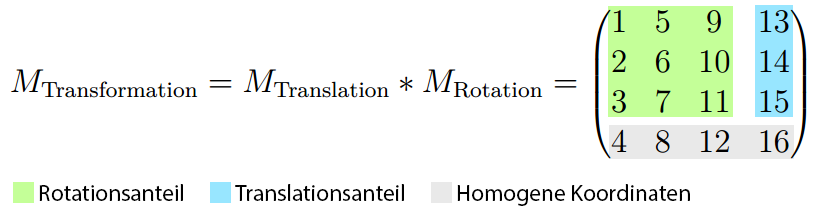
\includegraphics[width=120mm]{bilder/transformationsmatrix.png}
\caption{Bestandteile der homogenisierten Transformationsmatrix}
\label{fig:transformationsmatrix}
\end{figure}

Der Server wandelt den TransformRequest in eine JSON-Struktur um und sendet diese über das Socket zurück an den Client. Sobald alle Knoten durchlaufen wurden, sendet der SirisOverlord die Nachricht \textit{NodeSetupComplete} an den OsirisMessagEvaluator zurück, welcher diese in ein JSON umwandelt und an den Client schickt. Der Client registriert dies und fährt mit der Vorbereitung für das Rendering fort.

\section{Benutzereingaben verarbeiten}
Über die Tastatur soll der Benutzer mit der Szene interagieren können. Da Szenen sehr unterschiedlich aufgebaut sein können, muss in der Szene hinterlegt sein welche Tastendrücke was bewirken. Zu diesem Zweck wurde in der Szene ein Knoten vom Typ "`keyboard"' hinterlegt, welcher die aktivierbaren Tasten und die daraufhin auszuführenden Aktionen in einer Keymap beschreibt. Das hierfür notwendige Modul heißt \textit{HandleUserInput}. Um die Modellknoten verändern zu können, müssen innerhalb des Moduls Referenzen auf diese vorgehalten werden. Zudem verwendet es das \textit{SendMessageToServer}-Modul, um die auszuführenden Aktionen (derzeit nur \textit{ApplyImpulse}) an den Server schicken und die Antworten verarbeiten zu können. Listing \ref{lst:userinput} zeigt den Code um auf Benutzereingaben reagieren zu können. Das \texttt{\$}-Zeichen ist die Factory-Methode der \textit{Zepto}-Bibliothek.
\lstset{language=JavaScript}
\begin{lstlisting}[caption={Reaktion auf Benutzereingaben}, label={lst:userinput}]
$(document).keydown(function(event) {
  var manipulationRequest = node.keyMap[event.which];

  if (manipulationRequest) {
    SendMessage.execute(new Msg.ManipulationRequest(manipulationRequest.nodeId, manipulationRequest.type, manipulationRequest.data), _onServerResponse);
  }
});
\end{lstlisting}
Wenn der Anwender eine Taste drückt die eine Aktion hervorrufen soll, wird mit den in der Keymap hinterlegten Daten ein neuer \textit{ManipulationRequest} erzeugt und an den Server gesendet. Listing \ref{lst:transformrequest} zeigt den Ablauf bei einer Antwort des Servers.
\lstset{language=JavaScript}
\begin{lstlisting}[caption={Reaktion auf Benutzereingaben}, label={lst:transformrequest}]
var nodeToTransform;

if (response.status === "transform") {
  nodeToTransform = _nodesToHandle[response.data.nodeId];
  nodeToTransform.transformation = response.data.transformation;
}
\end{lstlisting}
Bei einer gültigen Antwort (der Status ist "`transform"') wird der zu transformierende Modellknoten über die zurückgelieferte ID in der Map \texttt{\_nodesToHandle} gesucht. Anschließend wird seine gegenwärtige Transformationsmatrix durch die in der Servernachricht enthaltene ersetzt.

\section{Darstellen der Szene}
Vor dem Rendering muss festgelegt werden welche Daten mit welchem Zweck an das Shaderprogramm gebunden werden. Dieses Binden ist notwendig, da weder der Renderer noch das Shaderprogramm wissen können, ob und wie die in der Szene enthaltenen Daten mit den Attributes und Uniforms in den Shadern assoziiert sind. Wie bereits beschrieben enthält die vom Server zurückgelieferte Shaderprogrammkonfiguration auch Informationen über die bindbaren Attributes und Uniforms. Das Modul \textit{SetupShaderBindableLocations} sucht diese im Shaderprogramm und speichert ihre Referenzen in einem \texttt{locations}-Objekt. Dies wird später in der Rendering-Schleife verwendet um relevante Daten, wie die Vertices eines 3D-Modells oder Texturinformationen, an die Shader zu übertragen. Im Modul \textit{RenderScene} wird anschließend die Rendering-Schleife ausgeführt. In WebGL kann hierfür die Funktion \texttt{requestAnimationFrame} verwendet werden, welche für jedes gerenderte Bild aufgerufen wird. Diese Funktion bietet zudem noch einige Komfortfunktionen. Sollte der aktuelle Tab oder Fenster beispielsweise nicht mehr sichtbar sein weil der Benutzer einen anderen Tab oder Fenster geöffnet hat, wird die Animationsschleife nicht mehr ausgeführt. Dies reduziert die Belastung der Hardware und spart Energie. Der Browser kann noch weitere Optimierungen vornehmen, je nachdem wie der Browserhersteller die Funktion implementiert hat. Da der Name der Funktion noch nicht in allen Browser standardisiert ist, wurde auch hierfür die WebGL Utils-Bibliothek verwendet.
\begin{figure}
\centering
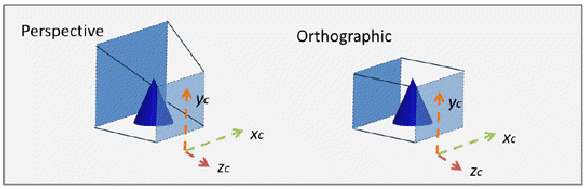
\includegraphics[width=\textwidth]{bilder/views.png}
\caption{Links: der kegelförmige Sichtraum der Perspektivischen Projektion, Rechts: der quaderförmige Sichtraum der Orthographischen Projektion\autocite{WebGLBeginnersGuide}}
\label{fig:views}
\end{figure}

Zur Darstellung der Szene verwendet der Renderer zwei Matritzen:
\begin{enumerate}
    \item \textbf{Modelviewmatrix}\\
Die Modelviewmatrix ist die kombinierte Matrix aus der Model- (3D-Objekt) und der Viewtransformation (Kamera) in der Szene. Sie bestimmt die Position und Ausrichtung jedes Objekts in der Szene und ist daher von besonderer Bedeutung.
    \item \textbf{Projektionsmatrix}\\
Die Projektionsmatrix bestimmt wie die Szene dargestellt wird. Hierzu sind zwei Projektionsarten möglich: In der Orthographischen Projektion bleiben parallele Linien parallel und Objekte behalten, unabhängig von ihrer Entfernung zum Betrachter, ihre proportionale Größe. In der Perspektivischen Projektion hingegen werden Objekte die vom Betrachter weiter entfernt sind kleiner gezeichnet. Die Perspektivische Projektion ergibt ein realitätsgetreueres Bild.
\end{enumerate}
Auf die Relevanz dieser Matrizen wird weiter unten bei der Beschreibung der Vorgänge für jeden Knoten näher eingegangen.
\lstset{language=JavaScript}
\begin{lstlisting}[caption={Implementierung der Lookup-Tabelle für das Rendering}, label={lst:lookuptable}]
var _lookupTable = {
  "renderInformation": _updateRenderer,
  "camera": _updateViewport,
  "ambientLight": _updateAmbientLight,
  "pointLight": _updatePointLight,
  "model": _renderModel
};
\end{lstlisting}
Da der gesamte Rendering-Vorgang recht komplex ist wurde hierfür ein extra Modul namens \textit{TraverseAndRender} hinzugefügt. In jeder Iteration der Renderschleife wird die Szene darin einmal traversiert und je nach gefundenem Knotentyp gehandelt. Die Traversierung erfolgt rekursiv. Für jeden gefundenen Knoten wird ein registriertes Callback ausgeführt. Das Callback entscheidet dann anhand des Knotentypen wie mit diesem verfahren werden muss. Um längere Entscheidungsbäume und damit potenzielle Leistungseinbußen zu vermeiden wurde hierfür eine Lookup-Tabelle verwendet (siehe Abbildung \ref{fig:lookupvergleich}).
\begin{figure}
\centering
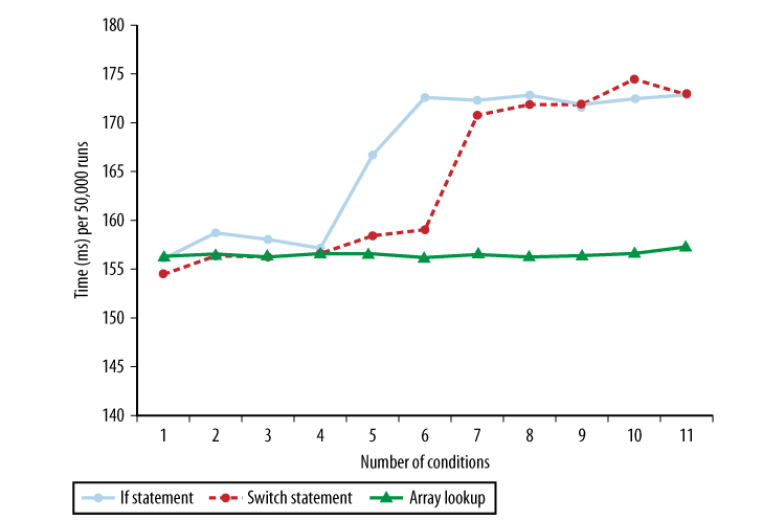
\includegraphics[width=\textwidth]{bilder/lookup_vergleich.png}
\caption{Leistungsvergleich Lookup-Table, If-Else und Switch im IE 7 \autocite{HighPerformanceJS}}
\label{fig:lookupvergleich}
\end{figure}
Diese ist ein einfaches JavaScript-Objekt, in dem der Knotentyp die auszuführende Funktion referenziert (siehe Listing \ref{lst:lookuptable}).
Sobald der gefundene Knotentyp in der Lookup-Tabelle gefunden wurde, wird die dort referenzierte Funktion ausgeführt. Für die folgenden Knoten sind Funktionen registriert.

\subsection{Modellknoten}
Für jeden Modellknoten wird versucht mindestens die Vertices und Indizes im Vertexshader zu binden, da diese die Mindestanforderung darstellen um das Modell zeichnen zu können. Indizes definieren die Faces (Oberflächen) des 3D-Modells explizit, indem sie die Reihenfolge der zu zeichnenden Dreiecke angeben. Andere Rendermodi als \texttt{TRIANGLES} werden vom Renderer nicht unterstützt. Sollten jedoch weitere Informationen, wie die Normalen, Texturkoordinaten, Texturen etc. vorhanden sein, werden diese ebenfalls über die im \texttt{locations}-Objekt enthaltenen Referenzen an ihre jeweiligen Attributes bzw. Uniforms angebunden.

Um zu garantieren, dass jedes Modell in der Szene später unabhängig von anderen Objekten gezeichnet wird und nur auf es einwirkende physikalische Kräfte reagiert, wird vor dem Zeichnen eine Kopie der aktuelle Modelviewmatrix auf einem Stack abgelegt. Die originale Modelviewmatrix wird mit der aktuellen Transformationsmatrix des Objekts multiplitziert, wodurch das Objekt genau an der Position und mit der Ausrichtung gezeichnet wird, die von seiner Transformationsmatrix vorgegeben wird. Nach dem Zeichenvorgang wird die originale Modelviewmatrix wieder vom Stack geladen und so verhindert, dass die Transformation des vorherigen Objektes Einfluss auf das nachfolgende hat.

In den Modellknoten können Materialeigenschaften wie \texttt{diffusecolor} oder Texturen hinterlegt werden. Je Knoten sind eine Color und eine Specular Map möglich.

\subsection{Kameraknoten}
Wie OpenGL ES hat auch WebGL kein dediziertes Kameraobjekt. Um ein solches zu simulieren ist die Projektionsmatrix von besonderer Bedeutung. Der Renderer unterstützt sowohl die Orthographische als auch die Perspektivische Projektion. Die Art der Projektion wird im "`camera"'-Knoten in der Szene eingestellt. Für das Einstellen der Projektionsart bietet die \textit{glMatrix}-Bibliothek die Hilfsfunktionen \texttt{perspective} und \texttt{ortho} an. Im Eigenschaftsobjekt \texttt{optics} des Kameraknotens werden die notwendigen Informationen, wie beispielsweise Öffnungswinkel, Near und Far Plane, erwartet.

Auch für das Festlegen der Position, des Blickziels und der Ausrichtung der Kamera bietet die \textit{glMatrix}-Bibliothek eine Hilfsfunktion namens \texttt{lookAt}. Die hierfür notwendigen Informationen sind im Eigenschaftsobjekt \texttt{position} des Kameraknotens hinterlegt (siehe auch Abbildung \ref{fig:cam}). Auf diese Weise lassen sich alle für die Kamera relevanten Informationen auf menschenlesbare Weise in der Szene hinterlegen.
\begin{figure}
\centering
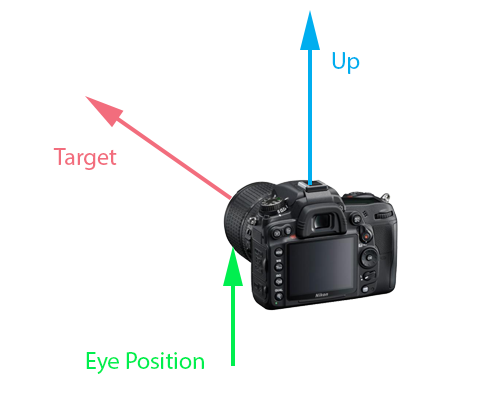
\includegraphics[width=80mm]{bilder/cam.png}
\caption{Relevante Vektoren der Kamera (Copyright des Kamerabildes: \copyright Nikon Corporation)}
\label{fig:cam}
\end{figure}
Damit der Rendering Canvas beim Vergrößern und Verkleinern des Browserfensters mitskaliert, wird die Größe des Canvas und das Ansichtsverhältnis bei jedem Durchlauf der Renderschleife neu berechnet.

\subsection{Renderinformationen}
Die für den Renderer relevanten Informationen werden im Knotentyp "`renderInformation"' hinterlegt. Hierzu gehören:
\begin{itemize}
    \item \textbf{Clear color}\\
Die RGB-Werte, mit denen der Color Buffer initial überschrieben wird.
    \item \textbf{Clear}\\
Die Buffer, die zurückgesetzt werden sollen. Dies muss als Integerwert angegeben werden. Die Buffer sind als Konstanten in WebGL hinterlegt, so ist der Wert für das \textit{COLOR\-\_BUFFER\-\_BIT} 16384. Sollen sowohl der Color Buffer als auch der Depth Buffer zurückgesetzt werden, ist der Wert 16640. Dies ist die Summe aus 16384 und 256 (\textit{DEPTH\-\_BUFFER\-\_BIT}) \autocite{WebGLSpec}.
\end{itemize}
Diese können somit beispielsweise über Anwendereingaben geändert werden, da sie in jedem Durchlauf der Renderschleife überprüft werden.

\subsection{Beleuchtungsknoten}
Der Renderer unterstützt die Festlegung der Werte für das ambiente Licht, sowie Punkt-, direktionale und Spotlichquellen. Die eigentliche Unterstützung hierfür muss natürlich im Shader eingebaut sein. Der Renderer weiß lediglich welche Daten für den jeweiligen Lichttyp mindestens benötigt werden und an das Shaderprogramm gesendet werden müssen. Es ist jeweils nur maximal ein Licht jeden Typs pro Szene verfügbar.